\section{Ejercicio 2}

\subsection{Introdución}
En esta sección se procede a realizar una máquina de estados capaz de detectar una secuencia de bits dada, siendo esta 1-1-0-1.

\subsection{Implementación} 
Para poder realizar este detector se consideró que el último bit de la secuencia puede ser el primero de una nueva, es decir, dada una cadena de bits de la forma 1-1-0-1-1-0-1, la máquina de estados detecta dos secuencias correctas de bits. También se consideró que, si un caracter es incorrecto, la el sistema vuelve a su estado base inicial, comenzando el proceso de nuevo. Es así que se realizo el siguiente diagrama de estados, utilizando una máquina de Mealy:
\begin{figure}[H]
\centering
	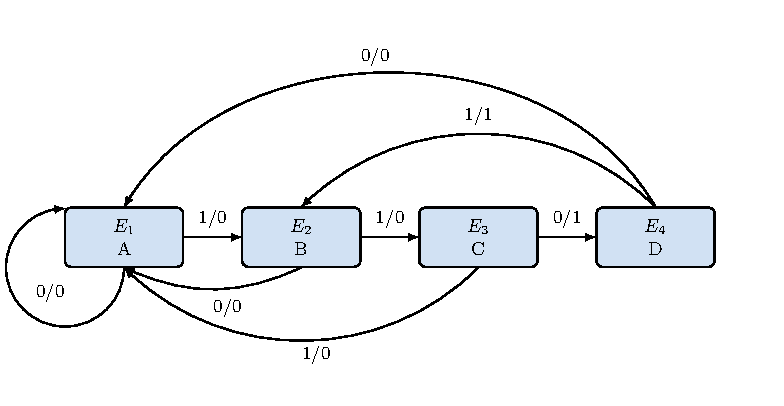
\includegraphics[width=0.7\textwidth, page = 1]{ImagenesEjercicio2/FSM2.pdf}
	\caption{Diagrama de la máquina de Mealy utilizada para detectar la secuencia de bits.}
\end{figure}

Se le otorgó a los estados la siguiente numeración: $A=00$, $B=01$, $C=10$, $D=11$. Es así que se obtiene la siguiente tabla:
\begin{table}[H]
\centering
\begin{tabular}{ccccc}
\hline
\multirow{2}{*}{Estado actual} & \multicolumn{2}{c}{Próximo estado} & \multicolumn{2}{c}{Salida} \\
 & w=0 & w=1 & w=0 & w=1 \\
\hline
$y_2y_1$ & $Y_2Y_1$ & $Y_2Y_1$ & $Z$ & $Z$ \\
A & A(00) & B(01) & 0 & 0 \\
B & A(00) & C(10) & 0 & 0 \\
C & D(11) & A(00) & 0 & 0 \\
D & A(00) & B(01) & 0 & 1 \\
\hline
\end{tabular}
\caption{Tabla de estados de la máquina de Mealy.}
\label{tab:estadosmealy}
\end{table}

A partir de lo expuesto en la Tabla (\ref{tab:estadosmealy}), se realizaron los respectivos mapas de Karnaugh para las salidas $Y_1$ e $Y_2$. Es así que se pudo observar que, tanto para los maxterminos como para los minterminos, el número de operaciones lógicas a realizar son las mismas, por lo tanto se optó por utilizar los minterminos, obteniendo así los siguientes mapas:
\begin{figure}[H]
\centering
\begin{subfigure}{0.45\textwidth}
	\centering
	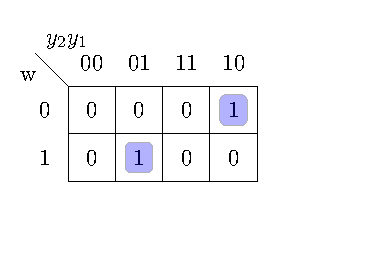
\includegraphics[width=\textwidth, page=1]{ImagenesEjercicio2/Mapas-Kar.pdf}
	\caption{Mapa del primer Flip-Flop.}
\end{subfigure}
\begin{subfigure}{0.45\textwidth}
	\centering
	\includegraphics[width=\textwidth, page=2]{ImagenesEjercicio2/Mapas-Kar.pdf}
	\caption{Mapa del segundo Flip-Flop.}
\end{subfigure}
\begin{subfigure}{0.5\textwidth}
	\centering
	\includegraphics[width=\textwidth, page=3]{ImagenesEjercicio2/Mapas-Kar.pdf}
	\caption{Mapa de la salida deseada.}
\end{subfigure}
	\caption{Mapas de Karnaugh implentados.}
	\label{fig:karnmealy}
\end{figure}

Con los mapas presentados en la Figura (\ref{fig:karnmealy}) se obtienen las siguientes funciones:
\begin{equation*}
	Y_1=(w\bar{y_2}\bar{y_1})+(wy_1y_2)+(\bar{w}y_2\bar{y_1})
\end{equation*}
\begin{equation*}
	Y_2=(w\bar{y_2}y_1)+(\bar{w}y_2\bar{y_1})
\end{equation*}
\begin{equation*}
	Z=wy_2y_1
\end{equation*}

Se emplean 2 flip-flops tipo D para representar las 4 combinaciones posibles, obteniendo así todos los estados posibles, considerando a su vez que los futuros pueden representar tanto la entrada y la salida de los flip-flops como el estado actual. Es así que se presenta el siguiente circuito:
\begin{figure}[H]
\centering
	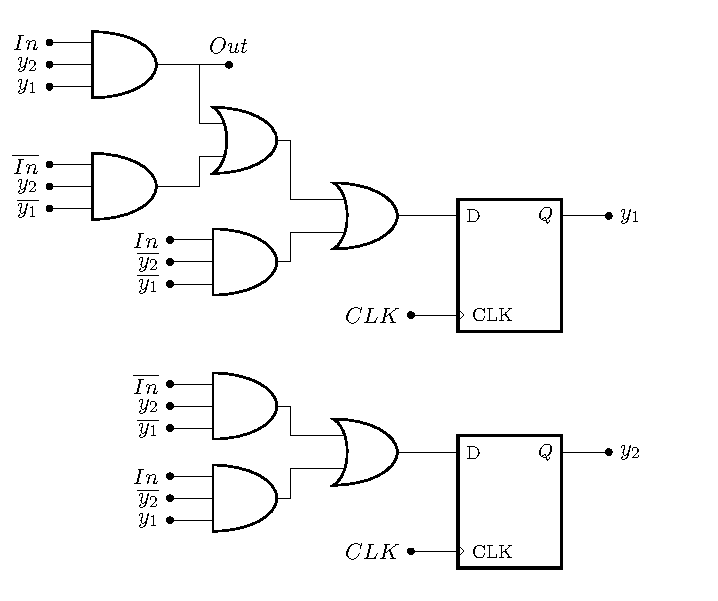
\includegraphics[width=0.6\textwidth, page=1]{ImagenesEjercicio2/Circuitos2.pdf}
	\caption{Circuito implementado.}
\end{figure}

Consecuentemente, se procedió a realizar la simulación en Verilog de dicho circuito. De esta forma se obtuvieron los siguientes resultados:
\begin{figure}[H]
\centering
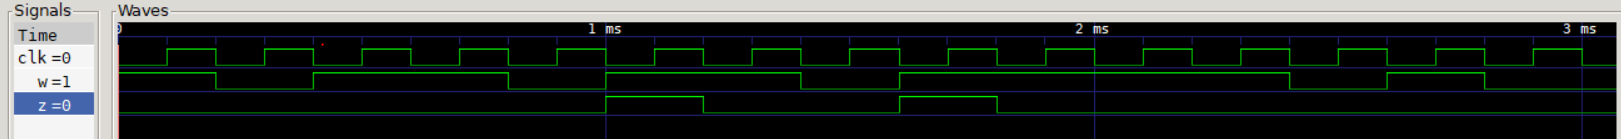
\includegraphics[width=0.9\textwidth]{ImagenesEjercicio2/simulacion.png}
\caption{Simulaciones en GTKwave, donde w simboliza la entrada, z la salida y clk el clock del circuito}
\end{figure}

Como era de esperarse, dicho circuito emula satisfactoriamente la máquina de estados planteada, por lo que se puede detectar correctamente la secuencia de bits deseados cuando esta se presenta. Posteriormente a las simulaciones, se procedió a diseñar dicho circuito en PCB, con el cual se obtuvieron los mismos resultados, por lo que se corroboró el correcto funcionamiento de la máquina de estados implementada, como se puede presenciar en las siguientes figuras.
\begin{figure}[H]
\centering
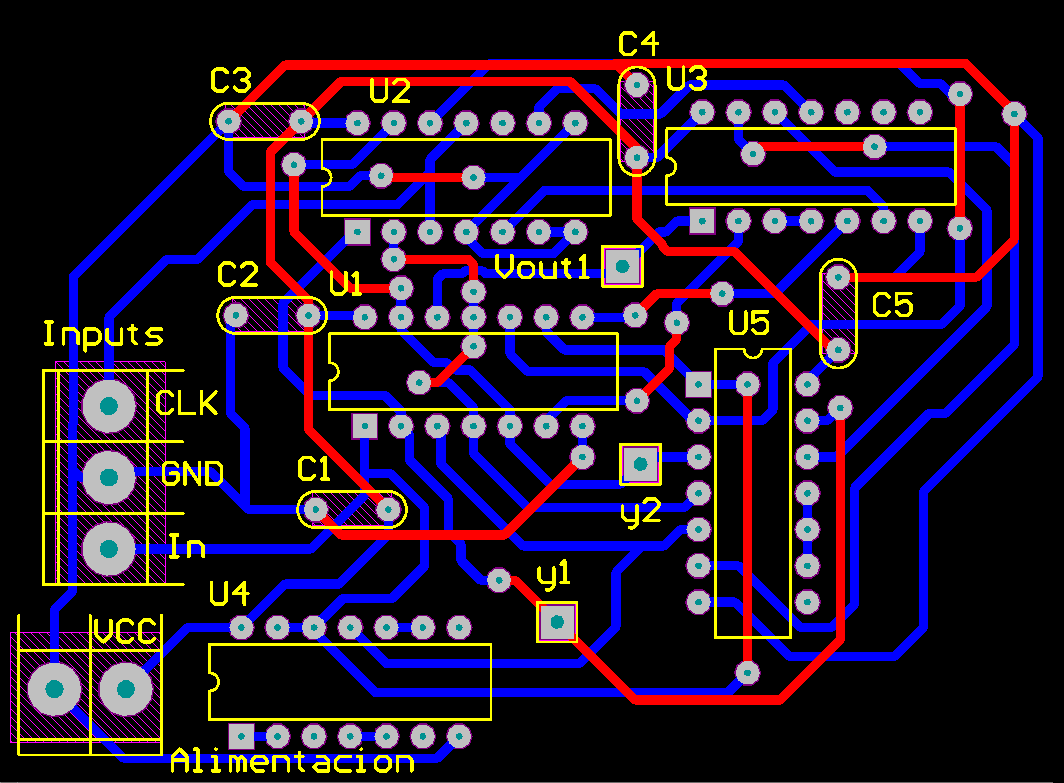
\includegraphics[width=0.7\textwidth]{ImagenesEjercicio2/pcb.png}
\caption{Implementación en PCB del circuito implementado.}
\end{figure}

\begin{figure}[H]
\centering
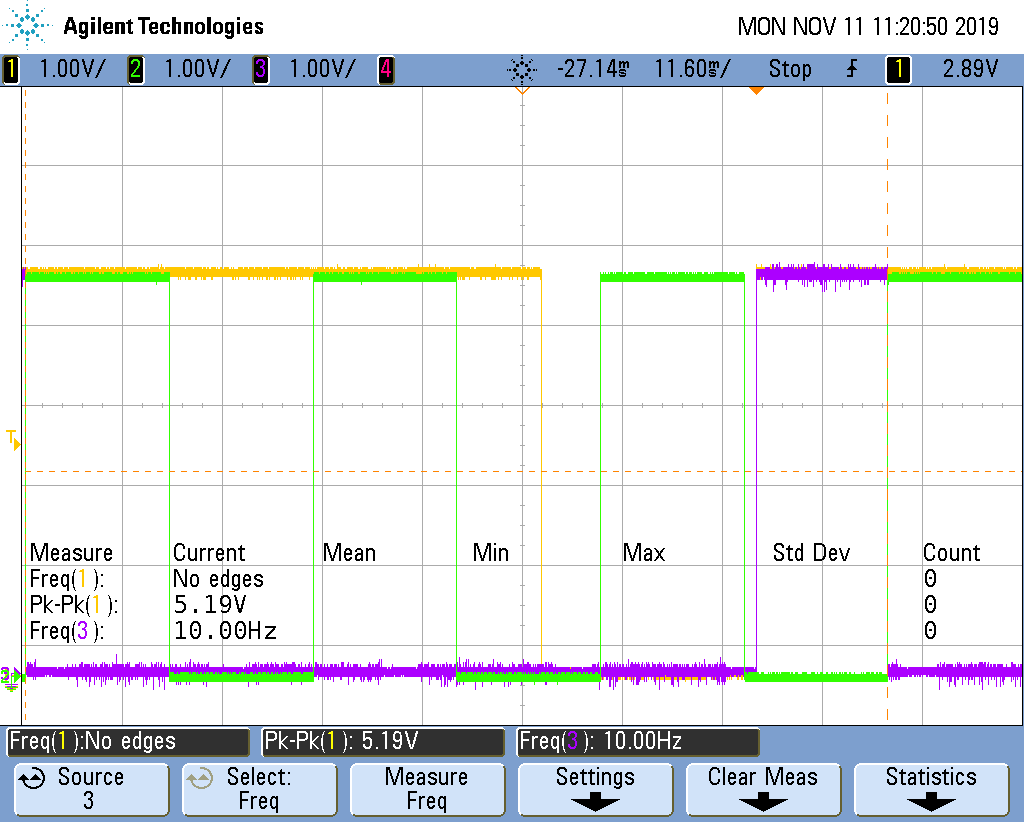
\includegraphics[width=0.6\textwidth,trim={0 2.2cm 0.1cm 1.75cm},clip]{ImagenesEjercicio2/scope_0.png}
\caption{Detección de la secuencia deseada vista en el osciloscopio.}
\label{fig:med-ej2}
\end{figure}

En la Figura (\ref{fig:med-ej2}) se presenta una medición de la detección de la secuencia deseada. En ella, se presentan en verde la señal de clock, en amarillo la señal de entrada y en violeta la salida. Además, es posible presenciar el funcionamiento de la maquina de estados. En ella, se presenta un desfasaje, en el que pareciera que la salida se logra en un estado bajo del clock. Dicha suposición es errónea, ya que esto se debe a que no se logró una sincronización entre la señal de entrada y el generador de clock. Dichas señales, a su vez, dado que la señal de salida pose una frecuencia distinta, se dificulta la captura de esta en el osciloscopio a un mismo tiempo, por lo tanto, se produce dicho desplazamiento entre las 3 señales.